\section{Applications}
\label{sec:application}
%%
The proposed technique benefits any visualization application which implicitly runs range distribution queries on the data. Applications mainly run three types of distribution queries:
%%
\begin{itemize}
%%
\item \emph{Random:} Interactive exploration of the spatial domain by the user is an example which places queries in random locations and sizes in no particular order.
\item \emph{Blockwise:} Some applications partition the data into blocks and require the distribution of each block as a substitute of downsampled data. Examples which compute low resolution approximate isosurfaces~\cite{Hixel11} or streamlines from distributions, or visualizations that present blocks clustered by their distributions~\cite{transgraph11} fall in this category.  Blockwise queries become difficult to answer when the application (or the user) demands blocks of a different size.
\item \emph{Pointwise:} Many applications compute and analyze statistical properties such as mean, variance and information entropy~\cite{Xu10} from distributions computed based on a local neighborhood at each point. Computation of pointwise queries across large domains is expensive, since it requires raw data access, as the query range or the per-voxel neighborhood size is changed.
%%
\end{itemize}

Our method seamlessly integrates with any visualization application which falls in one or more of the above three categories. Instead of accessing the raw data to answer each query, we use our method to retrieve the distributions faster. Following two subsections show two such applications.
%%
%%
%%\subsection{Analysis of Local Statistics}
%%\label{sec:application_1}
%%
%%
%% 
%%
%%
%%%%%%%%%%%%%%%%%%%%%
%% Diagram begins
%%%%%%%%%%%%%%%%%%%
%\begin{figure}[!htb]
%\centering
%	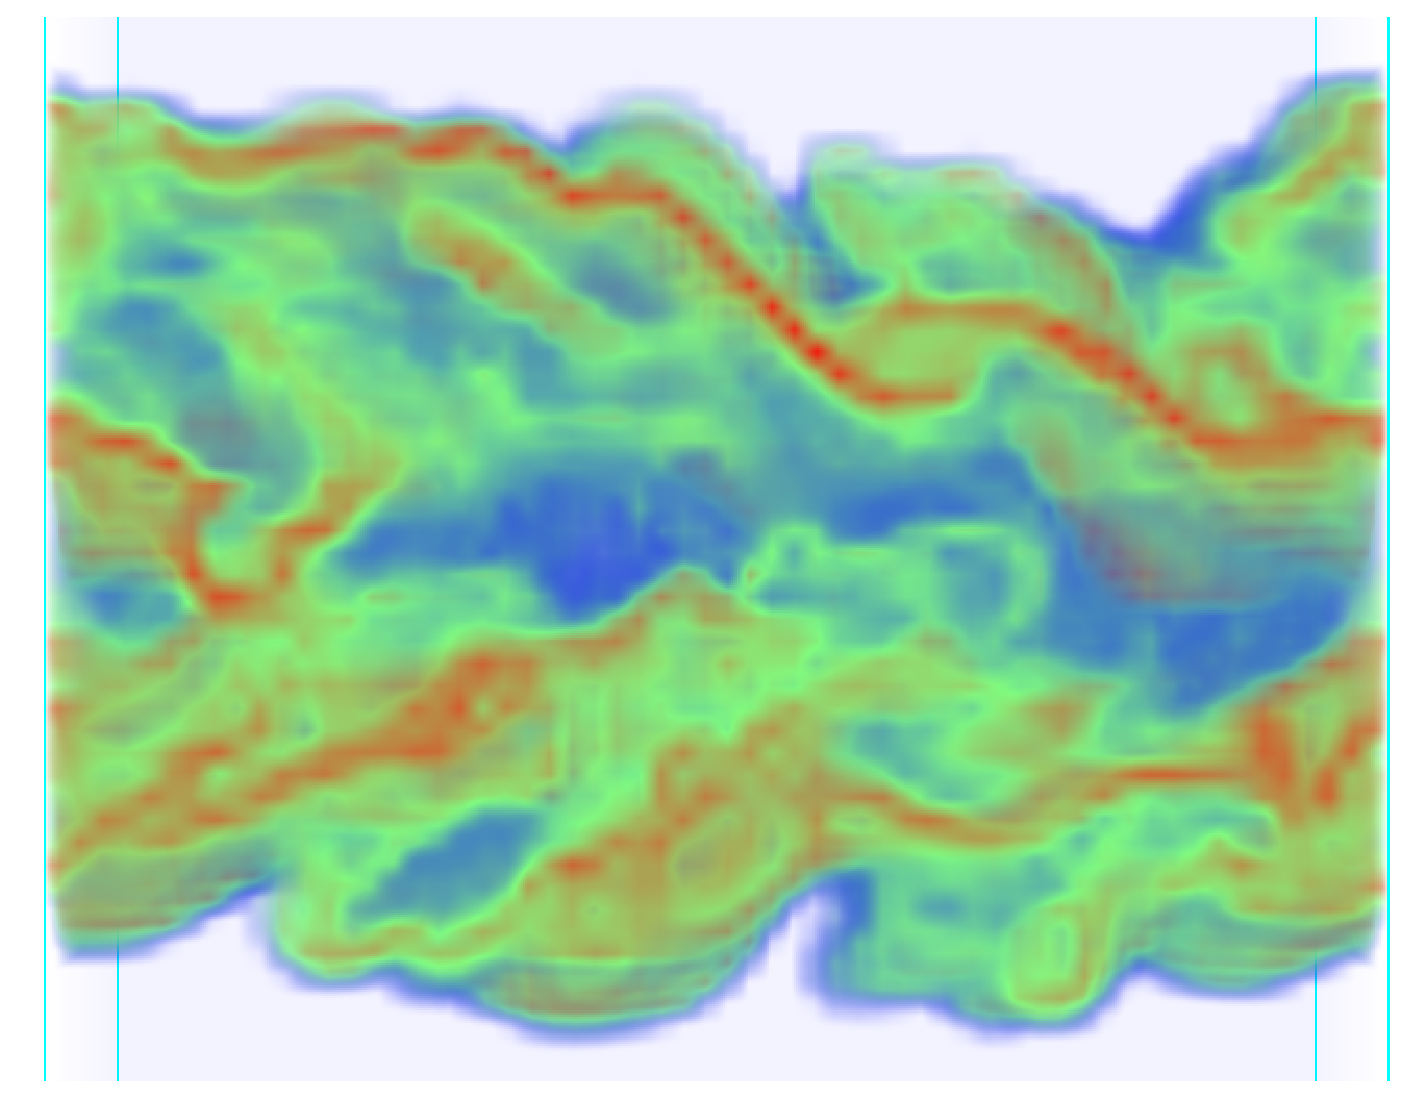
\includegraphics[width = 0.3\linewidth, keepaspectratio = true]{images/eps/mixfrac_entropy.eps}
%	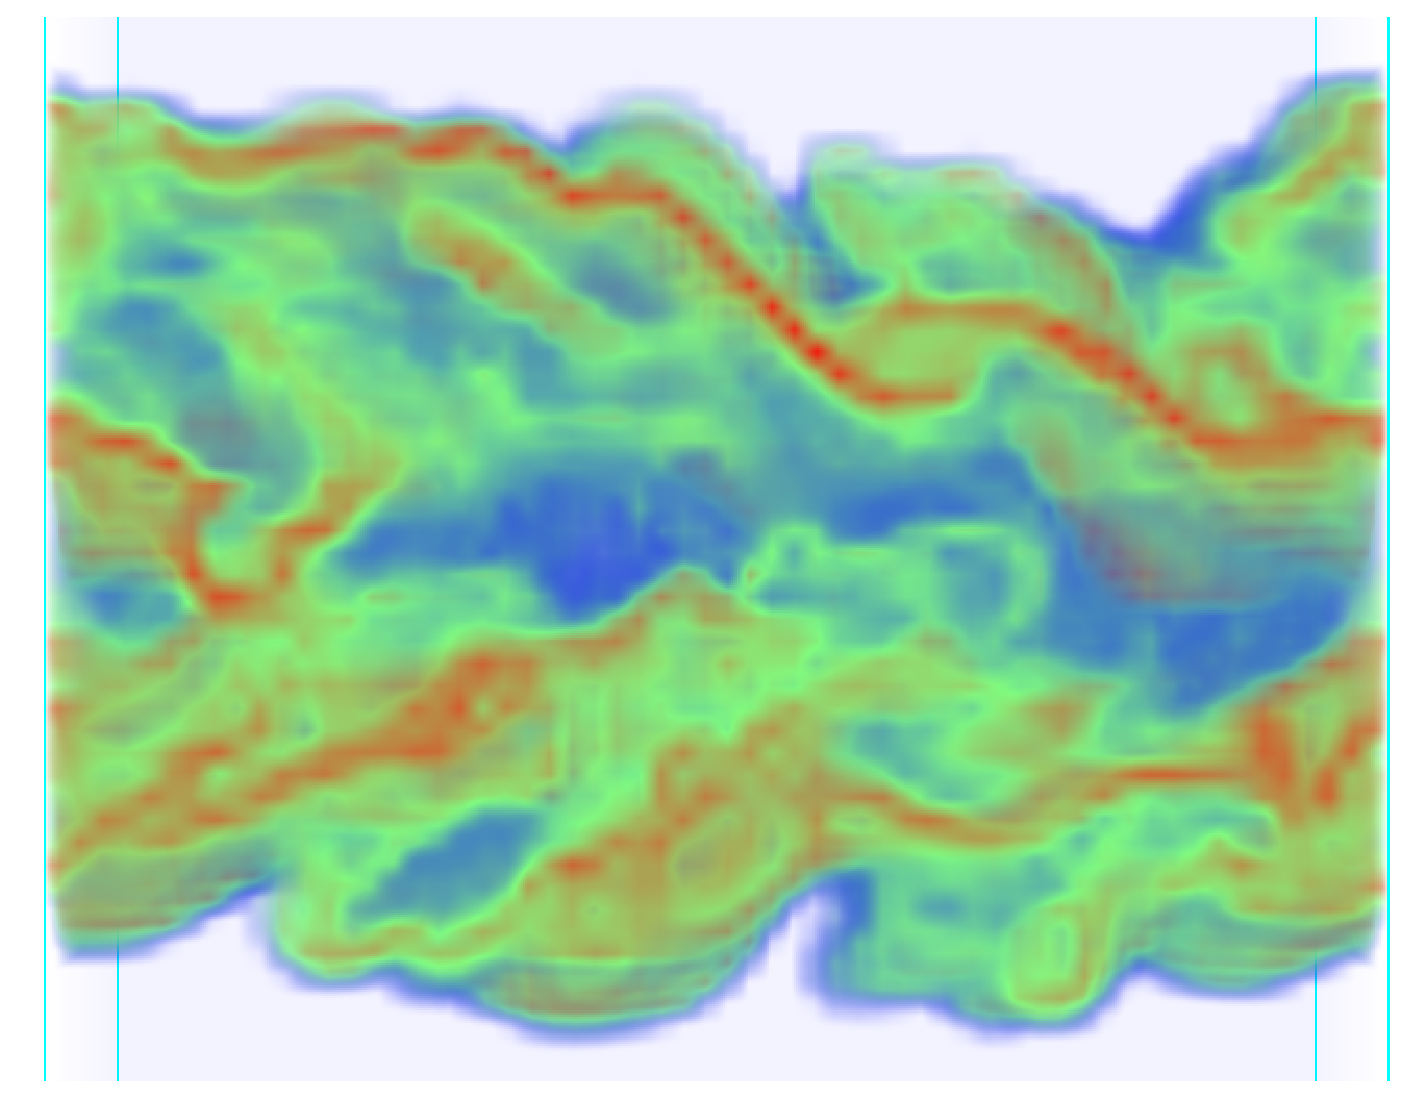
\includegraphics[width = 0.3\linewidth, keepaspectratio = true]{images/eps/mixfrac_entropy.eps}
%	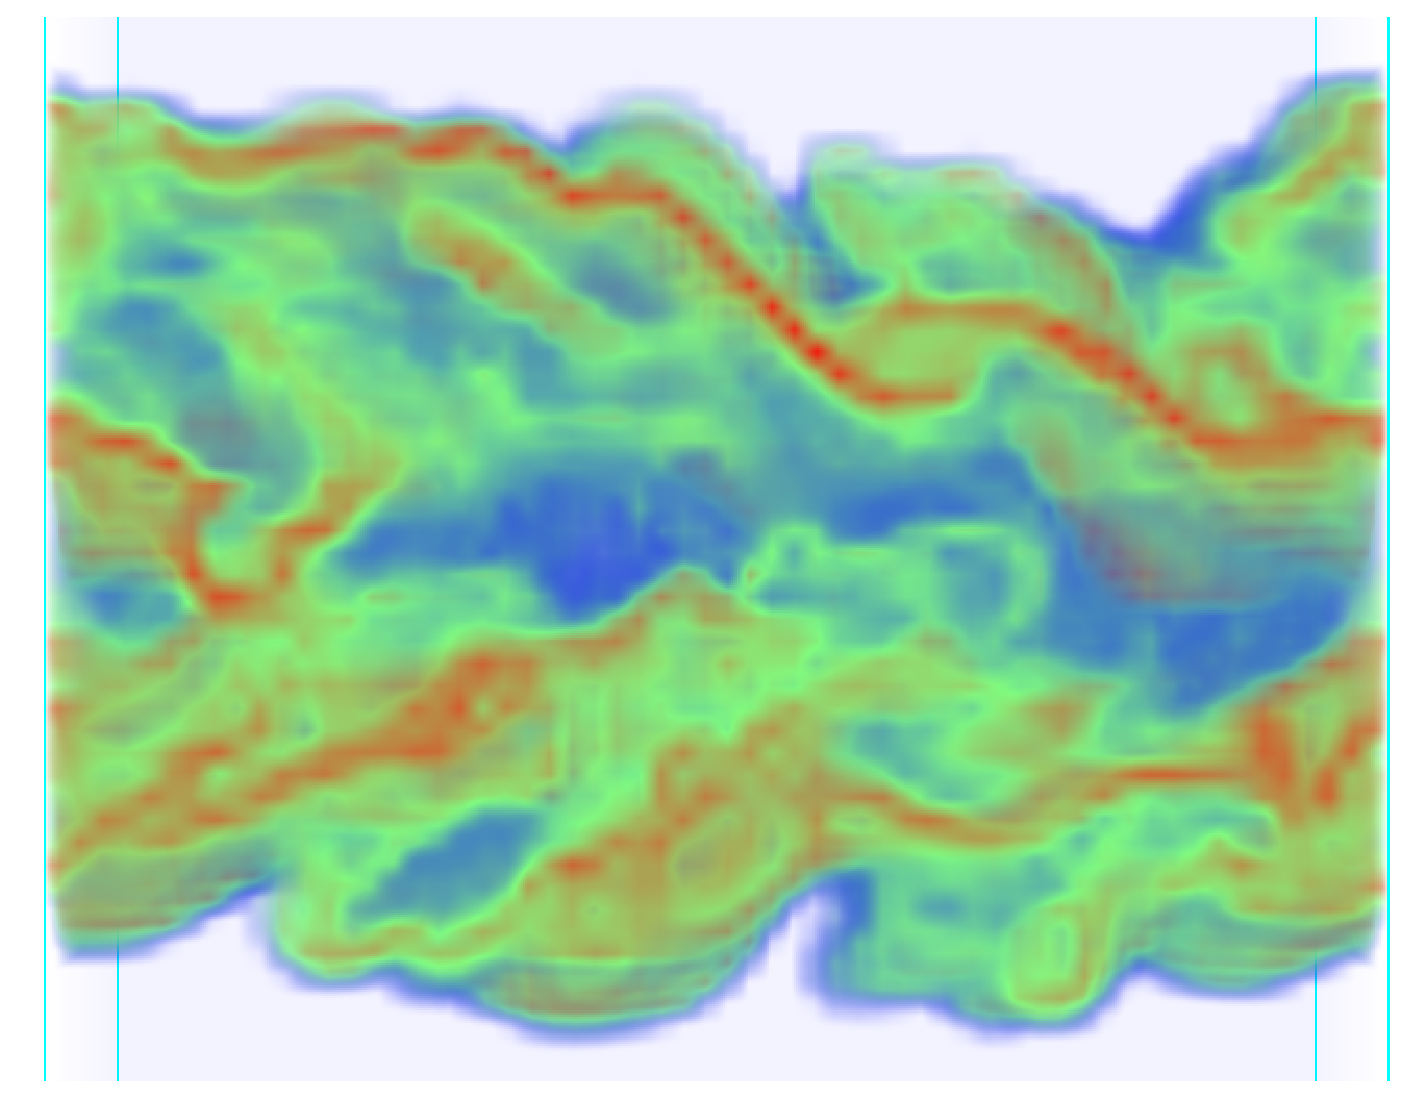
\includegraphics[width = 0.3\linewidth, keepaspectratio = true]{images/eps/mixfrac_entropy.eps}
%	\caption{Pointwise entropy field for different neighborhood sizes. {\bf *** Middle and right image will change ***}}	
%	\label{fig:localstat}
%	%\vspace{0.3cm}
%%\end{figure}
\begin{figure}[tb]
		\centering
		%\subfloat[Distribution based fuzzy isosurface computation for arbitrary resolutions from Isabel Pressure field. {\bf Left.} True isosurfaces. {\bf Middle Column} Volume rendering of likelihood field for block size 4. {\bf Right column} Likelihood field for block size 12.]
		%{\label{fig:fuzzysurface_isabel}
			\includegraphics[width = 0.64\linewidth, keepaspectratio = true]{images/eps/testcase_isabel_1.eps}
		%}
		\caption{Block distribution-based fuzzy isosurface computation for arbitrary levels of detail from Isabel Pressure field. {\bf Top.} True isosurfaces. {\bf Middle.} Likelihood field for -500 Pa. {\bf Bottom.} Likelihood fields for +100 Pa.}	
		\label{fig:fuzzysurface_isabel}
		\vspace{-0.1in}
\end{figure}		
%%%%%%%%%%%%%%%%%%%
%% Diagram ends
%%%%%%%%%%%%%%%%%%%

%We have employed our technique to compute such fields while varying the block size over a range. Figure~\ref{fig:localstat_plot} compares our method's performance against the raw data access method. Clearly, our method's does not depend on the neighborhood size used, while the raw data access method does. 
%%
%%
\subsection{Feature Detection with Fuzzy Isosurfaces}
\label{sec:application_1}
%%
%%
%%%%%%%%%%%%%%%%%%%
%% Diagram begins
%%%%%%%%%%%%%%%%%%%
%\begin{figure*}[tb]
%	\begin{minipage}{\linewidth}
%		\centering
%		\subfloat[Distribution based fuzzy isosurface computation for arbitrary resolutions from Isabel Pressure field. {\bf Left.} True isosurfaces. {\bf Middle Column} Volume rendering of likelihood field for block size 4. {\bf Right column} Likelihood field for block size 12.]
%		{\label{fig:fuzzysurface_isabel}
%			\includegraphics[width = 0.32\linewidth, keepaspectratio = true]{images/eps/testcase_isabel_1.eps}
%		}
%		~
%		\subfloat[Distribution-based search for different patterns on Solar Plume dataset (using a $9^3$ local neighborhood). {\bf Top.} A commonly occurring distribution and {\bf Bottom.} a sparsely present distribution used as template.] 	
%		{\label{fig:fuzzysearch_plume}
%			\includegraphics[width = 0.32\linewidth, keepaspectratio = true]{images/eps/similaritysearch_plume.eps}
%		}
%		\subfloat[Distribution-based search for different patterns on Solar Plume dataset (using a $9^3$ local neighborhood). {\bf Top.} A commonly occurring distribution and {\bf Bottom.} a sparsely present distribution used as template.] 	
%		{\label{fig:fuzzysearch_plume}
%			\includegraphics[width = 0.32\linewidth, keepaspectratio = true]{images/eps/similaritysearch_combustion.eps}
%		}
%	\end{minipage}	
%	\\
%	\begin{minipage}{0.38\linewidth}
%		\centering
%				\subfloat[Performance improvement: local statistics computation. {\bf ***Plot spaceholder***}]	
%		{\label{fig:localstat_plot}
%			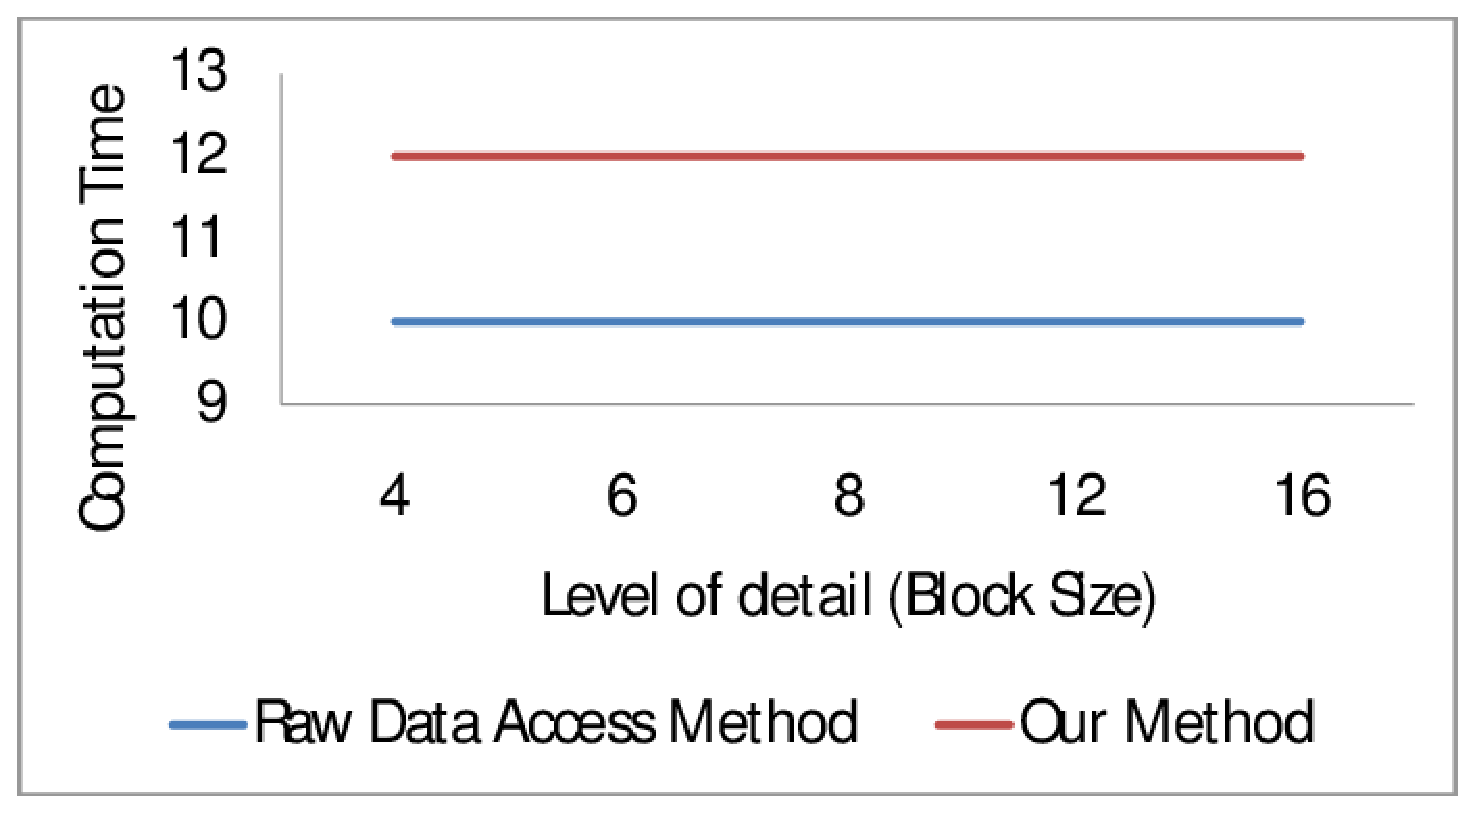
\includegraphics[width = 0.3\linewidth, keepaspectratio = true]{images/eps/plot1.eps}
%		}		
%		~
%		\subfloat[Performance improvement: local statistics computation. {\bf ***Plot spaceholder***}]	
%		{\label{fig:localstat_plot}
%			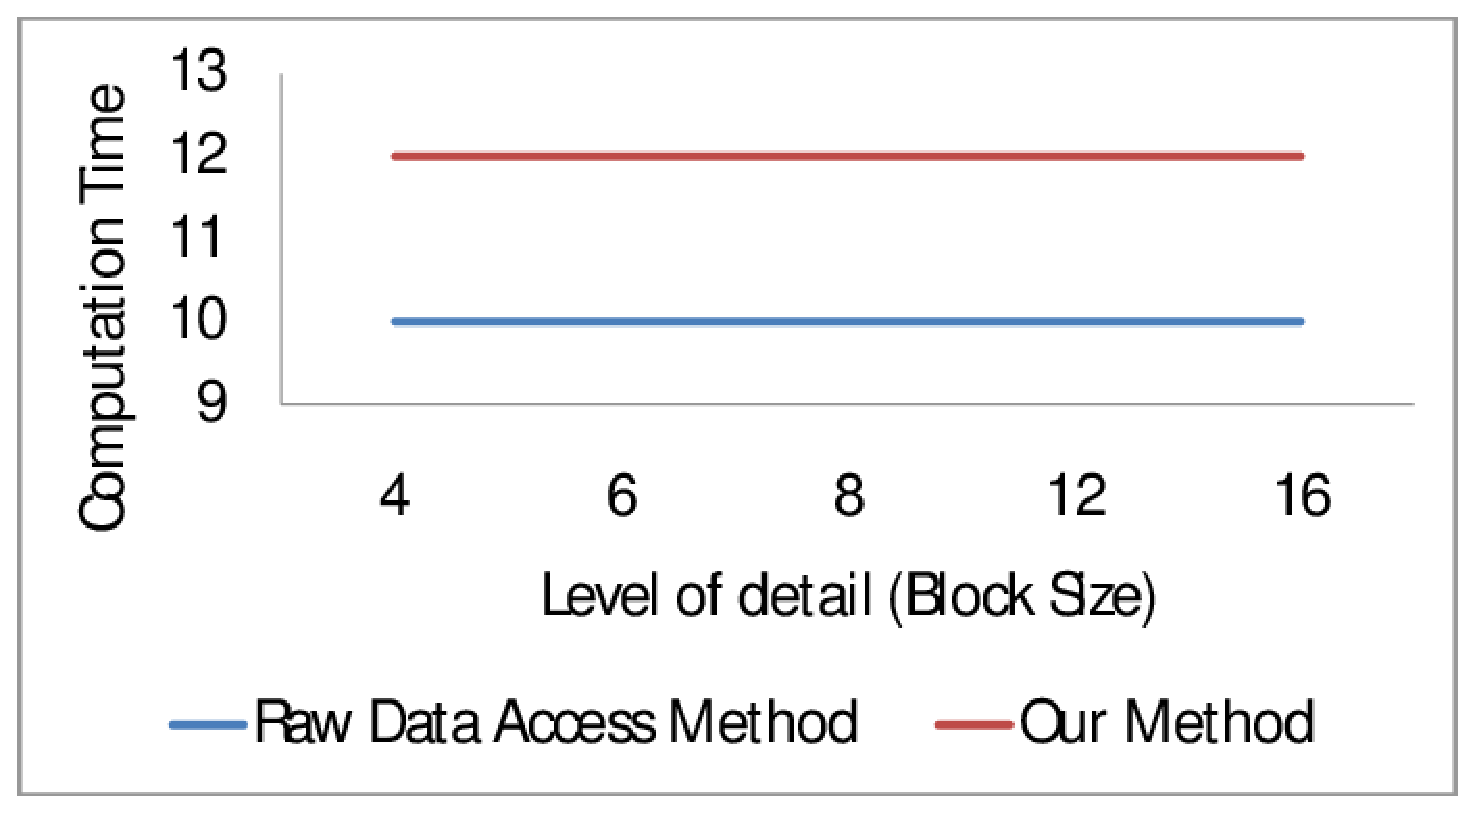
\includegraphics[width = 0.3\linewidth, keepaspectratio = true]{images/eps/plot1.eps}
%		}		
%		~
%		\subfloat[Performance improvement: Fuzzy isosurface {\bf ***Plot spaceholder***}]	
%		{\label{fig:fuzzyiso_plot}
%			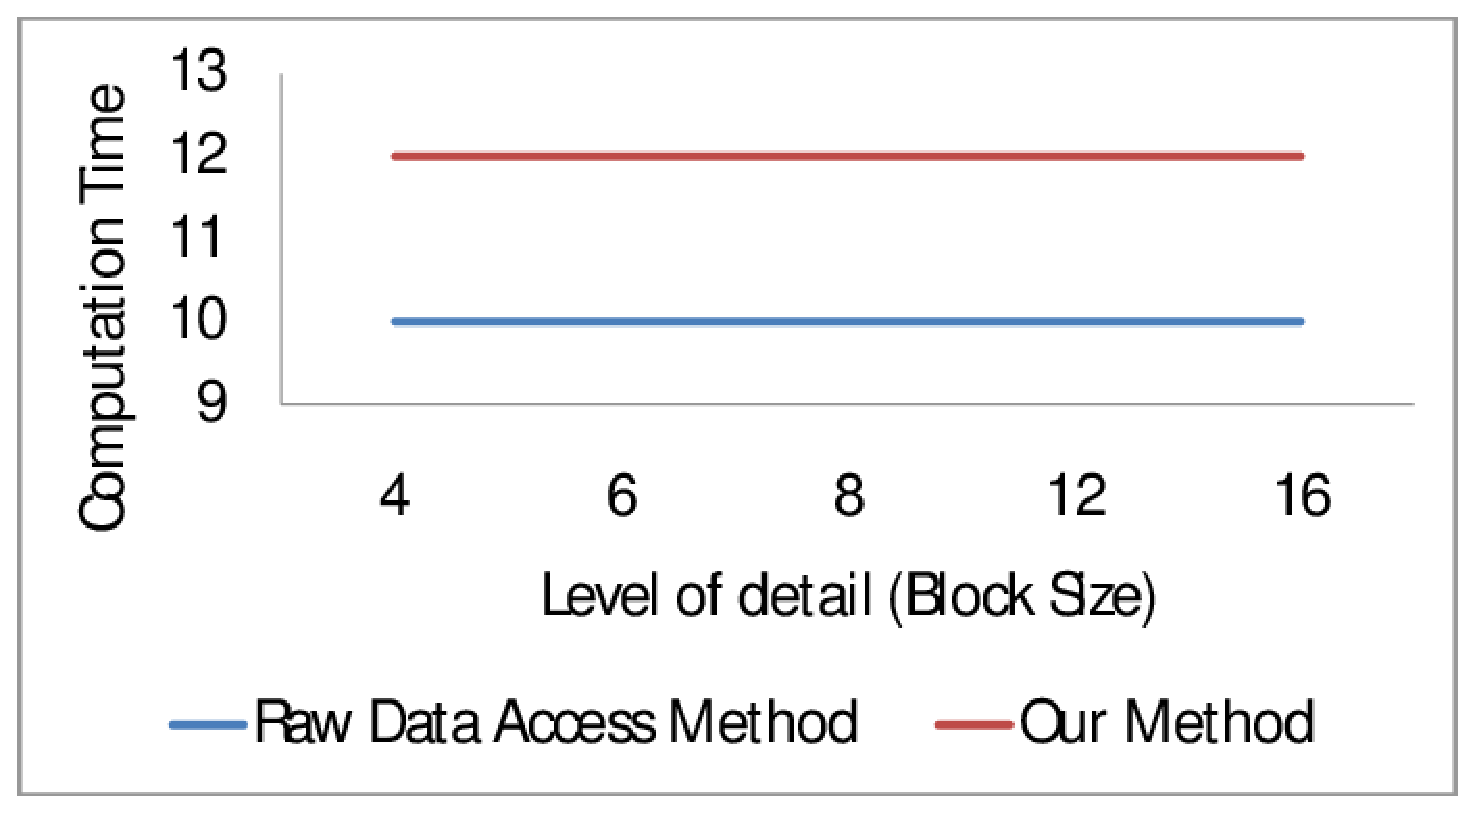
\includegraphics[width = 0.3\linewidth, keepaspectratio = true]{images/eps/plot1.eps}
%		}			
%	\end{minipage}	
%%	~
%%	\begin{minipage}{\linewidth}
%%		\centering
%%		~
%%		~		
%%		\subfloat[Performance improvement: Fuzzy similarity search {\bf ***Plot spaceholder***}]	
%%		{\label{fig:fuzzysearch_plot}
%%			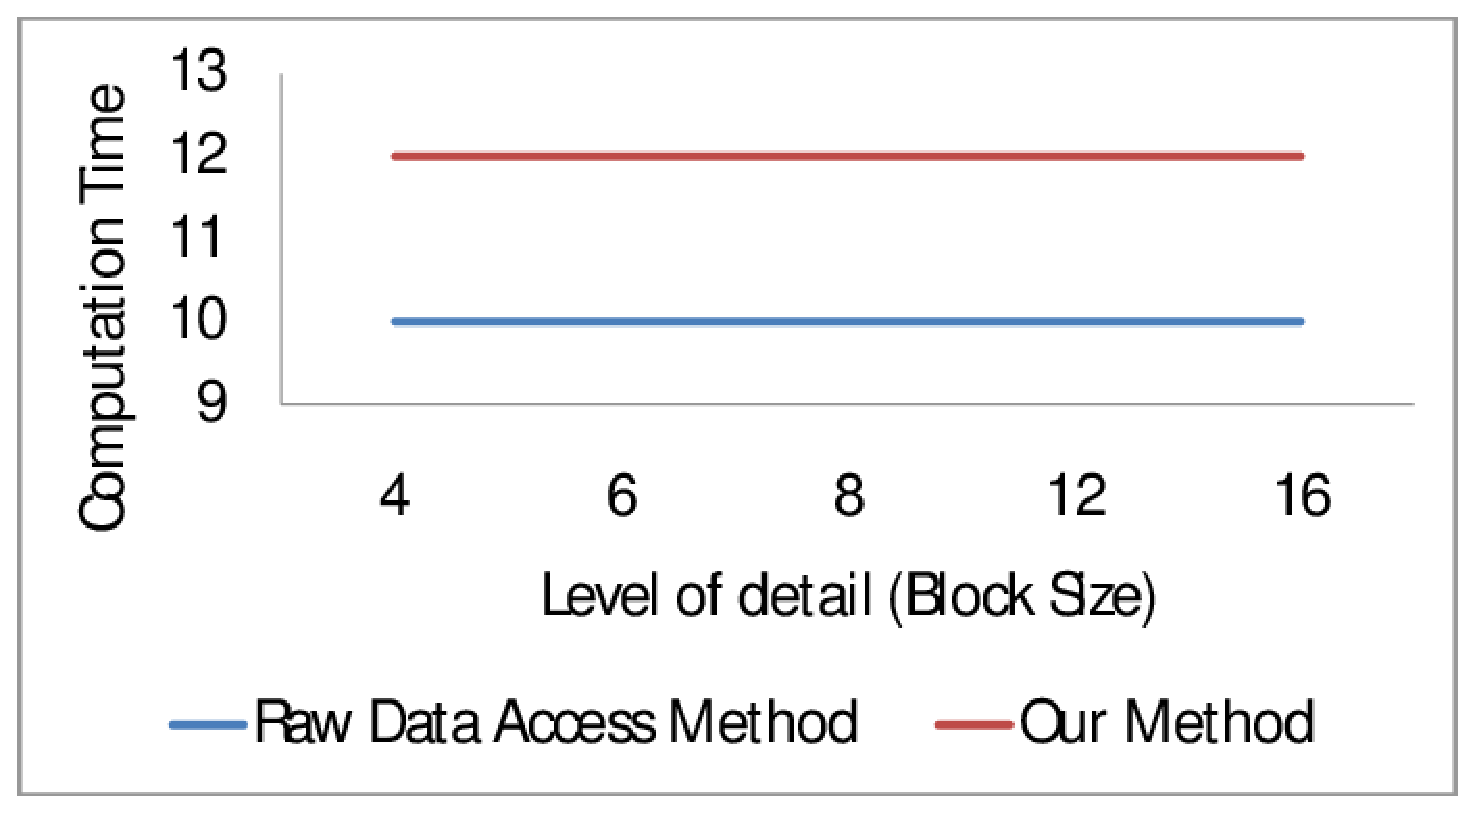
\includegraphics[width = 0.3\linewidth, keepaspectratio = true]{images/eps/plot1.eps}
%%		}		
%%
%%	\end{minipage}	
%
%	\caption{Estimation of various summary statistic using encoded distributions.}
%	
%	\label{fig:applications}	
%\end{figure*}
%%%%%%%%%%%%%%%%%%%
%% Diagram ends
%%%%%%%%%%%%%%%%%%%
%%
We first present an application which runs blockwise distribution queries. Thompson et. al.~\cite{Hixel11} has shown that, in the presence of large-scale data, fuzzy isosurfaces computed from block-level distributions retain the main features present in the original data. When raw data is not available, their technique computes a \emph{likelihood value} for each block for a given isovalue. In the resulting field, zero indicates maximum likelihood of an isovalue being present in a block. However, depending on the required precision and available resources, the user often wants the ability to compute and visualize these likelihood values at different levels of detail. This either requires repeated data access to compute distributions for blocks of varying sizes, or requires storage of pre-computed distributions for a range of block sizes which can easily exceed the data size. Both are impractical for large data. \\
%%
%%%%%%%%%%%%%%%%%%%
%% Diagram begins
%%%%%%%%%%%%%%%%%%%
\begin{figure}[tb]
	\centering
	\subfloat[Distribution-based search on Solar Plume.] 	
	{\label{fig:fuzzysearch_plume}
	\includegraphics[width = 0.7\linewidth, keepaspectratio = true]{images/eps/similaritysearch_plume.eps}}\\
	\subfloat[Distribution-based search on Combustion.] 	
	{\label{fig:fuzzysearch_combustion}
	\includegraphics[width = 0.7\linewidth, keepaspectratio = true]{images/eps/similaritysearch_combustion.eps}}
	\caption{ (a) Distribution-based search for different patterns on Solar Plume dataset (using a $9^3$ local neighborhood). A commonly occurring distribution {\bf (top)}, and a sparsely present distribution {\bf (bottom)} used as template. (b) Distribution-based search for locations with stoichiometric mixture rate of 0.42 on time step 118 of combustion dataset (using a $7^3$ local neighborhood).}
	\label{fig:fuzzysearch}	
	\vspace{-0.1in}
\end{figure}	
%%%%%%%%%%%%%%%%%%%
%% Diagram ends
%%%%%%%%%%%%%%%%%%%

In this situation, our method can fast retrieve the block distributions for any level of detail on demand, without touching the raw data and having to store a large number of distributions. For example, at block size 32, our method finishes a set of 200 block-based queries in 0.11 seconds while the raw data access method takes 2.62 seconds (detailed performance study is in Section~\ref{subsec:analysis_encoding_space}). 

We have shown one example using the pressure field of hurricane Isabel dataset. According to previous research~\cite{qdv11}, pressure values less than -350 Pa correspond to the hurricane eye. The top image in Figure~\ref{fig:fuzzysurface_isabel} shows the  true isosurface for isovalue -500 Pa, (blue surface), which surrounds the hurricane eye, and the isosurface for +100 Pa (orange surface), which spans a large area outside the eye. The middle row contains the likelihood field for isovalue -500 Pa computed from block sizes 4 and 12. The bottom row shows the likelihood fields for +100 Pa for blocks of size 4 and 12. The importance of using different block sizes becomes apparent from the images. For isovalue -500 Pa, having the ability to use higher level of detail is necessary, since it indicates a localized feature with a distinct shape. On the other hand, a bigger block size may be sufficient for understanding isovalue +100 Pa, which does not represent or contain a fine feature. 
%%
%%
\subsection{Distribution-based Similarity Search}
\label{sec:application_2}
%%
%%
The second application is an example of pointwise range distribution query. When the user does not know the exact isovalue to look for, it is more convenient to place the query in the form of a distribution, a Gaussian kernel centering at the best estimated isovalue or a Gaussian mixture for example. If a feature is characterized by a particular type of distribution, that also prompts the user to search for that type of distribution in the data. In this context, Johnson and Huang~\cite{johnson09} has proposed to compute a \emph{fuzzy similarity score} which indicates the similarity between the user-input distribution and a local neighborhood based distribution at each voxel. The resulting similarity field has a score range from 0 to 1, 1 indicating the best match. However, whenever the query changes or the neighborhood size to be used for search changes, this method has to re-compute the distributions at each voxel. Doing this by accessing the raw data becomes very slow since it involves multiple accesses to the every data point. For example, our method computes pointwise distributions at every 4th point (based on a $32^3$ local neighborhood, query set contains total 48.8K points) of \emph{mixfrac} variable of combustion data in 6.15 seconds, while the raw data access method takes 186.65 seconds. 

Figure~\ref{fig:fuzzysearch_plume} shows two examples of distribution based search on Solar Plume. The query for the top image (distribution shown in inset) is a more common one, so most voxels of the resulting field have higher similarity score (red or orange) and only a few regions are dissimilar to the query (shown in blue). On the contrary, the query distribution for the bottom image is a Gaussian mixture where both Gaussians are centered at less probable values. Hence, most of the voxels in the similarity field are 0 or close to 0 (shown in blue). We have modulated the opacity to highlight the two small regions corresponding to the two Gaussian peaks in the query. Figure~\ref{fig:fuzzysearch_combustion} shows a distribution query on mixture fraction variable of Combustion data. We have used a Gaussian distribution centered at 0.42 as the query. The high similarity zones in the search result (red, right image) correspond well to the flame extinction zones (value $\sim$0.42) in the raw data (red, left image).


